\graphicspath{{survey-methods/}}

\chapter{Introducing our survey methods}
\label{chap:survey}

Chapters~\ref{chap:evilndi}, \ref{chap:prondi}, and \ref{chap:mechanism} all
utilize similar survey methods to assess climate-related beliefs and attitudes,
in addition to a number of related constructs relevant to Ranney's
(\citeyear{ranney_why_2012}) RTMD theory. For reference, the full list of survey
items used in this body of research is included in
Appendix~\ref{app:survey-items}. Note that codes for each item are given in
\textsf{sans serif} typeface, and that convention will indicate these codes in
what follows. For example, one question has the code \textsf{knwgbl}. Codes
which include numbers, such as \textsf{gw1_2}, indicate that they are one of
several questions probing a particular construct (in this case, GW beliefs and
attitudes).  In our experimental chapters, we'll examine the way our
interventions are able to shift these beliefs and attitudes (primarily those
related to climate change), as well as noting how these beliefs and attitudes
relate to one another.  I hasten to note that the number of potential
relationships between the many variables we have measured would require an
enormous amount of data to test fully. As such, we will restrict ourselves
primarily to the exploration of \emph{a priori} relationships of interest.

\section{Clarifying \texorpdfstring{“beliefs”}{"beliefs"} and
    \texorpdfstring{“attitudes”}{"attitudes"}}

Survey methods in the social sciences may use the terms “belief” and “attitude”
in a quite technical fashion. For example, in Fishbein's Theory of Reasoned
Action, an “attitude” is essentially the weighted sum of a set of beliefs and
norms \parencite[see][for an overview of such theories]{montano_theory_2008}.
While we will not contradict this formulation, below we take a more
common-language approach. Specifically, in the text that follows, a “belief”
should be taken as a measure of agreement with an objectively verifiable fact
about the world (For example, the reality of anthropogenic climate
change (assessed primarily by item \textsf{gw1_2}) may be difficult to
ascertain, but in the end, it is something that could be settled by observation.
An “attitude,” on the other hand, indicates a measure of agreement with an
emotional or evaluative stance towards some aspect of the world.  For example,
worry about global warming (\textsf{gw2_3}).

\section{An overview of survey items}

Survey items were primarily sourced from \textcite{martinez_factors_2009}, and
were chosen on the basis of both observed quality (from the results of
\cite{martinez_factors_2009}) and conceptual fit for our interventions. The
first page in particular (consisting of the 6 items with a “1” prior to the
underscore) was selected as the most ideal set of 6 questions for targeting the
6 RTMD constructs, depicted in Figure~\ref{fig:rtmd}
\parencite{ranney_why_2012}.  Notably, \textsf{gw1_2} was selected for its focus
on acceptance of \emph{anthropogenic} climate change. Note that while we
included a variety of measures in our surveys, in what follows, we will focus
solely on those items assessing GW attitudes and beliefs.

\begin{figure}
    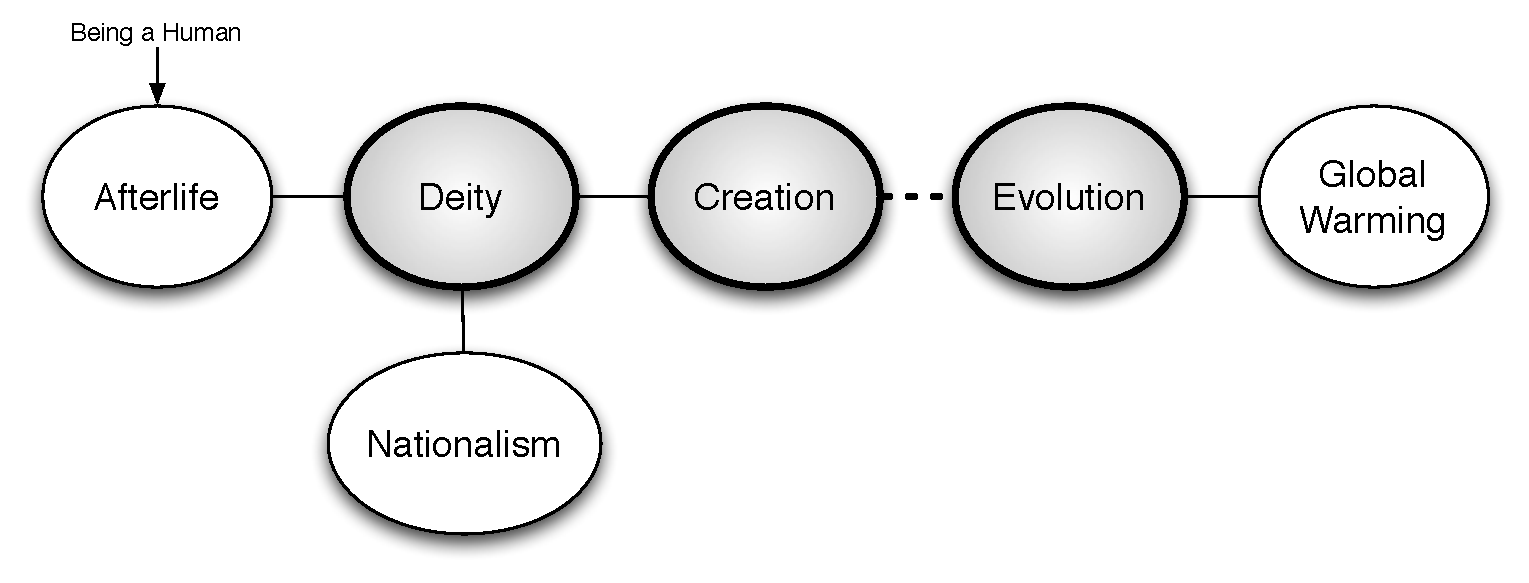
\includegraphics[width=6.5in]{rtmd.pdf}
    \caption{Core RTMD relationships (adapted from \textcite{ranney_why_2012}).
        Conceptual reinforcement (operationalized as positive correlation) is
        represented by a solid line, and conceptual incompatability by a dashed
        line. A coherent cluster representing devotion to “god and country” is
        on the left, and a science-accepting cluster is on the right. The most
        direct conflict is captured by the explanatory competition between
        creation and evolution. Note that while all constructs were surveyed,
        GW items are primarily eported on in this document.}
    \label{fig:rtmd}
\end{figure}

\subsection{Na\"ive survey results}

Most of the climate-related interventions that follow include some measure of
participant attitudes and beliefs prior to the intervention. In this
dissertation, we are primarily seeking insight into different forms of
conceptual \emph{change} (and thus, one hopes, behavioral change). Given this, a
detailed consideration of these na\"ive results is beyond our scope. However,
some of the relationships obtained seem relevant to understanding the mind of
our potential students. I thus note such results below. For a fuller treatment
of survey material, please consult the relevant publications of the Reasoning
group (notably, \cite{cohen_san_2012_f,ranney_changing_2012}).

\textcite{cohen_san_2012_f} reports a variety of results from a sample of 270
San Diego residents (270 park visitors and 69 community college students).
Notably, some important relationships were obtained using Cohen’s data contrary
to the “knowledge deficit” and polarization arguments referenced in
Section~\ref{sec:comm-strategies}. First, we observe a robust correlation
between mechanistic climate change knowledge and attitude toward climate change.
This result was maintained even when taking political party into account.
Specifically, mechanistic knowledge correlates with acceptance that global
warming is occurring ($r=0.22$, $p=0.0002$) and is anthropogenic ($r=0.17$,
$p=0.005$).  Anthropogenic climate change acceptance also predicted financial
“willingness to sacrifice” ($χ^2(4) > 32$, $p<0.001$ for each of four items),
and one’s knowledge score predicted two of these items ($χ^2(1) > 3.8$, $p<0.05$
for both). Further, acceptance of biological evolution was found to predict
beliefs and attitudes toward climate change (as RTMD hypothesizes, and, e.g.,
\cite{ranney_why_2012} found). 

We might infer, then, that “acceptance of controversial science” is a problem
above and beyond political ideology. These findings suggest that the effects of
well-chosen aspects of education are both significant and somewhat independent
of political affiliation. Indeed, evolution acceptance was a significant
predictor of climate change acceptance even in a model including the two major
political parties ($\chi^2(4)=12.3$, $p<0.02$; N.B., including other parties
dramatically reduces quality of fit for any model, likely due to small bin
sizes). Given these results with a representative sample of the american public,
we considered ourselves justified in focusing primarily on attitude and belief
questions in the interventions that follow.

Below, as appropriate, we will see how such relationships maintain
in our various populations in the context of a number of interventions.

% Include multi-correlation figures here?
% 
% Figure? Evo—GW link
% Knowledge / self-knowledge (this isn’t really part of this section)
% Other stuff? Maybe nationalism GW link? How does this tie generally into our
% theoretical framework? How does it compare and contrast with Ranney’s previous
% work?

\section{Ensuring quality of survey responses}
\label{sec:attitude-quality}

A central concern in large survey studies is determining if the surveys were
completed in good faith. We want to avoid including surveys that were filled out
in a random or incoherent way. Below, I explain a graphical method for identifying individuals who fall outside
of the normal variation in responses across survey items.

\subsection{A Graphical Method for checking Survey Quality}

We can represent participant responses in a raster plot, where each response
from an individual is represeted by a particular shade or color in a grid. Each
column represents a specific question and each row represents an individual. We
can then easily sort rows by the mean response of that participant, and columns
by mean response for that question. Plots are created using only items that
should be relatively coherent (e.g., all items dealing with religion, or climate
change). An example of this is given in Figure~\ref{fig:consistency}.

\begin{figure}
    \begin{center}
        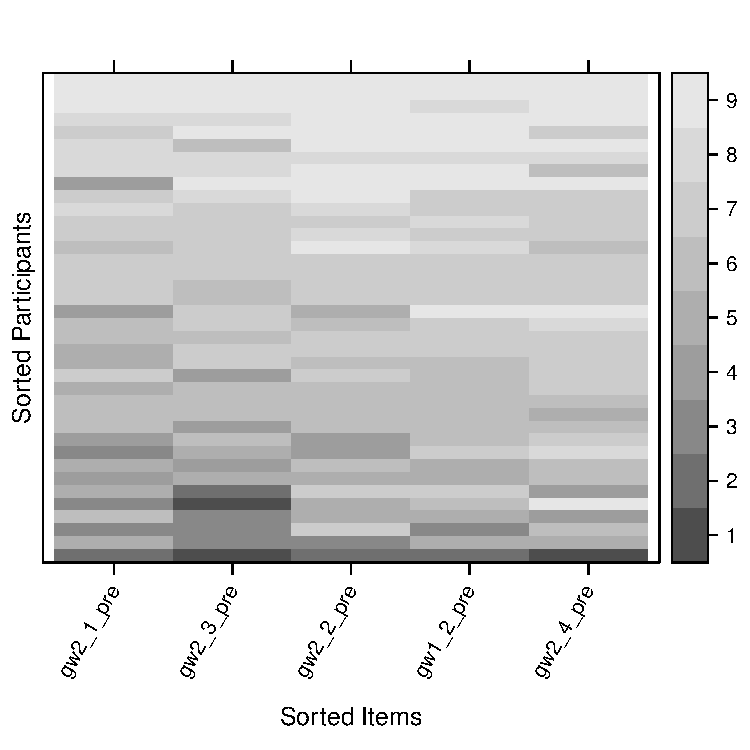
\includegraphics{consistency.pdf}
    \end{center}
    \caption{A plot allowing quick identification of individuals who answer
        markedly differently than those with similar mean attitudes. Here,
        \textsf{gw} items from the pre-test are plotted (reverse coded items are
        flipped prior to plotting). The item with the lowest mean rating is
        leftmost, and the item with the highest mean rating is rightmost.
        Likewise, participants are sorted in increasing mean order from bottom
        to top. The fifth individual from the bottom is a bit suspicious, with a
        “1” for \textsf{gw2_3} and a “9” for \textsf{gw2_4}, and thus was
        carefully inspected to ensure honest engagement with the survey. There
        are also two participants with straight “9”s at the top of the graph.
        Upon inspection, these participants simply provide extreme answers to
        all questions, but otherwise appear to be taking the survey seriously.}
    \label{fig:consistency}
\end{figure}

Participants who respond markedly differently from those with similar mean
scores pop out visually, and can be inspected manually. In many cases, after
inspection, such “abnormal” participants were retained---largely on the basis of
inspecting their written answers. Only if they appeared to be truly negligent or
outright non-cooperative in responding were they excluded. This method of
graphical inspection was applied for all samples in the following empirical
chapters, but may not be mentioned in cases where all subjects were considered
acceptable, as was normally the case.


\section*{Acknowledgements}

Particular thanks to Luke Miratrix for his input in developing the method
described in Section~\ref{sec:attitude-quality}.
